\documentclass[
%% TIKZ_CLASSOPTION %%
tikz
]{standalone}
\usepackage{amsmath}
\usetikzlibrary{matrix}
%% EXTRA_TIKZ_PREAMBLE_CODE %%
\begin{document}
%% TIKZ_CODE %%
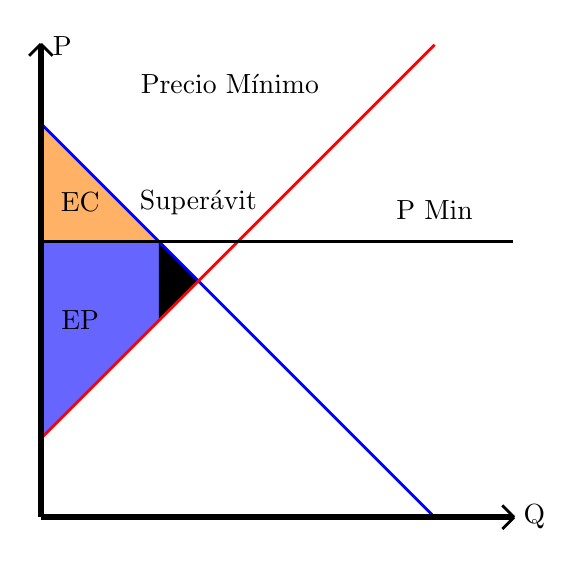
\begin{tikzpicture}

    % oferta = P(Q)=1+Q
    % demanda = P(Q)=5-Q
    
    
    % Etiquetas en el eje P
    % Area excedente del consumidor
    \fill[orange!60] (0,3.5) -- (0,5) -- (1.5,3.5) -- cycle;
    
    % Area excedente del productor
    \fill[blue!60] (0,1) -- (0,3.5) -- (1.5,3.5) -- (1.5,2.5) -- cycle;
    
    % perdida de eficiencia.
    \fill[black] (2,3) -- (1.5,3.5) -- (1.5,2.5) -- cycle;
    
    % demanda
    \draw [blue, line width=1pt](0,5) -- (5,0); %P(Q)=5-Q

    % oferta
    \draw [red, line width=1pt](0,1) -- (5,6); %P(Q)=1+Q
    
    \draw [line width=1pt](0,3.5) -- (6,3.5);
    
    % Eje x
    \draw[black, line width=2pt] (0,0) -- (5.98,0) node[right] {Q};
    \draw[black, line width=1pt] (5.86,-0.15) -- (6.01,0);
    \draw[black, line width=1pt] (5.86,0.15) -- (6.01,0);

    % eje y
    \draw[black, line width=2pt] (0,0) -- (0,5.98) node[right] {P};
    \draw[black, line width=1pt] (-0.15,5.86) -- (0,6.01);
    \draw[black, line width=1pt] (0.15,5.86) -- (0,6.01);

    %leyendas
    \node at (0.5,2.5) {EP};
    \node at (0.5,4) {EC};
    \draw (1.5,3.5) -- (2.5,3.5);
    \node at (5,3.9) {P Min};
    \node at (2,4) {Superávit};
    \node at (2.4,5.5) {Precio Mínimo};
    
\end{tikzpicture}
\end{document}
